% *******************************************************************************
% * Copyright (c) 2007 by Elexis
% * All rights reserved. This document and the accompanying materials
% * are made available under the terms of the Eclipse Public License v1.0
% * which accompanies this distribution, and is available at
% * http://www.eclipse.org/legal/epl-v10.html
% *
% * Contributors:
% *    G. Weirich
% *
% *  $Id: molemax.tex 1106 2008-12-30 13:59:09Z  $
% *******************************************************************************

\documentclass[a4paper]{scrartcl}
\usepackage{german}
\usepackage[utf8]{inputenc}
\usepackage{makeidx}
\makeindex

\usepackage[pdftex]{graphicx}
\DeclareGraphicsExtensions{.pdf,.jpg,.png}

\usepackage{floatflt}
\usepackage{wrapfig}
\usepackage[]{hyperref}
\usepackage{color}
\begin{document}
\title{MoleMax}
\author{Gerry Weirich}
\maketitle

\section{Einführung}
\textbf{Idee und Konzept:} Dr. med. Angela Brögli, PD Dr. med. Andreas Häffner
\bigskip

MoleMax ist ein Elexis\textsuperscript{\textregistered}-Plugin zur Aufzeichnung von Hautbildern und zur Dokumentation der Entwicklung von Hautveränderungen über die Zeit.
MoleMax benötigt Elexis 1.1.1 oder höher.
\section{Konfiguration}
MoleMax speichert die Bilder standardmässig nicht in der Datenbank, sondern in einem von Ihnen vorzugebenden Verzeichnis. Legen Sie dieses Verzeichnis irgendwo an, wo es von jedem PC aus, von dem Sie Zugriff auf die Bilder benötigen, zugänglich ist. Wählen Sie dann \textsc{Datei-Einstellungen-MoleMax} und geben Sie dort den Pfad zu diesem Verzeichnis an. Dies muss auf jedem zugreifenden PC separat erledigt werden, da der Pfad ja auf unterschiedlichen Computern unterschiedlich benannt werden kann.
(Das Verzeichnis 'bilder' auf dem Server kann auf PC1 als /mnt/server/bilder eingebunden sein, auf PC2 vielleicht als S:$\backslash$bilder)

\bigskip

Ausserdem benötigt ein Anwender bestimmte Rechte, um die Bilder sehen oder ändern zu dürfen (Es ist ja im Allgemeinen nicht notwendig, dass Praxispersonal Zugriff auf diese Bilddokumentationen hat). Es sind die Rechte \glqq Molemax/Bilder sehen\grqq{} bzw. \glqq Molemax/Bilder ändern\grqq notwendig, welche unter \textsc{Datei-Einstellungen-Gruppen und Rechte-Zugriffssteuerung} einzustellen sind (Vgl auch Kapitel 10.2 im Elexis-Handbuch).

\section{Standardsequenz einlesen}
Eine Standardsequenz von Aufnahmen besteht aus je drei Bildern von links, vorne, rechts und hinten, also jeweils 12 Aufnahmen. Machen Sie diese 12 Aufnahmen in genau dieser Reihenfolge mit einer Digitalkamera, und schliessen Sie die Kamera an den Computer an. Öffnen Sie die View 'MoleMax' (S. Abb. \ref{fig:mole1}) und ziehen Sie das erste Bild der Sequenz in das Teilfenster links oben.
\begin{figure}[htp]
    \begin{minipage}{0.45\textwidth}
        \centering
         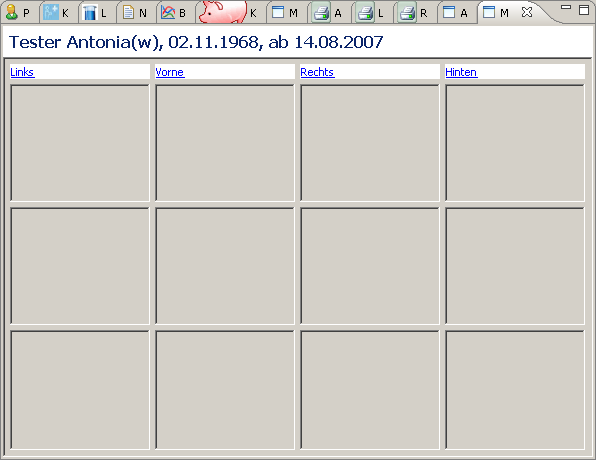
\includegraphics[width=0.9\textwidth]{molemax1}
         \hfill
         \caption{Leeres Molemax-Fenster}
         \label{fig:mole1}
     \end{minipage}
    \hfill
    \begin{minipage}{0.45\textwidth}
        \centering
         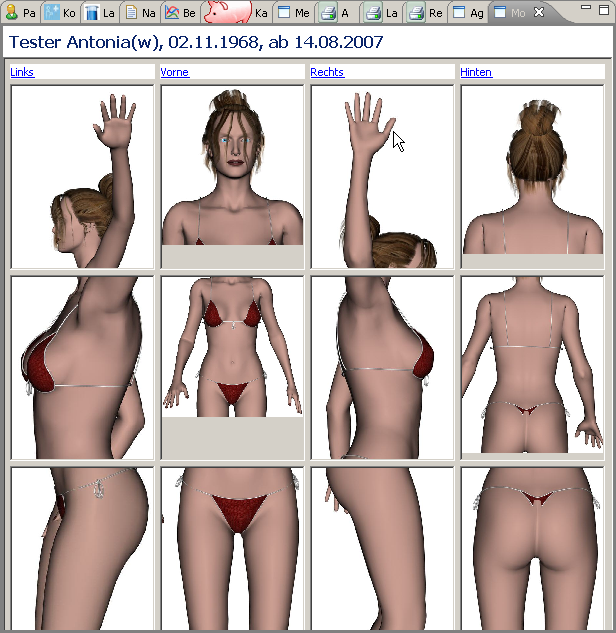
\includegraphics[width=0.9\textwidth]{molemax2}
         \caption{Serie eingelesen}
         \label{fig:mole2}
     \end{minipage}
\end{figure}

 Falls Ihre Kamera die Bilder aufeinanderfolgend numeriert hat, wird Elexis dann nachfragen, ob es die restlichen Bilder der Serie auch gleich einlesen soll. Dies geht nur dann gut, wenn die Bilder in der oben genannten Reihenfolge durchnumeriert sind. Andernfalls können Sie die Frage auch mit Nein beantworten und jedes Bild einzeln in das richtige Feld ziehen. Wenn Sie ein Bild falsch eingelesen haben, können Sie einfach ein anderes Bild an dieselbe Stelle ziehen, das vorherige Bild wird dadurch ersetzt.\footnote{Wenn Sie ein Bild wieder ganz entfernen möchten, klicken Sie mit der rechten Maustaste darauf und wählen aus dem Menü 'Löschen'}
Danach haben Sie ein Molemax-Fenster etwa wie in Abb \ref{fig:mole2}\footnote{Wenn Sie sich die nötigen Rechte zum Ansehen von Molemax-Bildern nicht gegeben haben (S. Konfiguration), werden Sie allerdings nur einen Text 'Rechte nicht ausreichend' sehen}.

Sie sehen oben an jeder Reihe einen Hyperlink mit der Aufschrift 'Links', 'Vorne', 'Rechts' und 'Hinten'. Klick auf den Hyperlink öffnet eine Detailansicht der betreffenden Reihe (Abb. \ref{fig:mole3})\footnote{Die Bilder unseres Modells Tester Antonia stammen von Daz3d}:

 \begin{figure}[htp]
     \begin{center}
         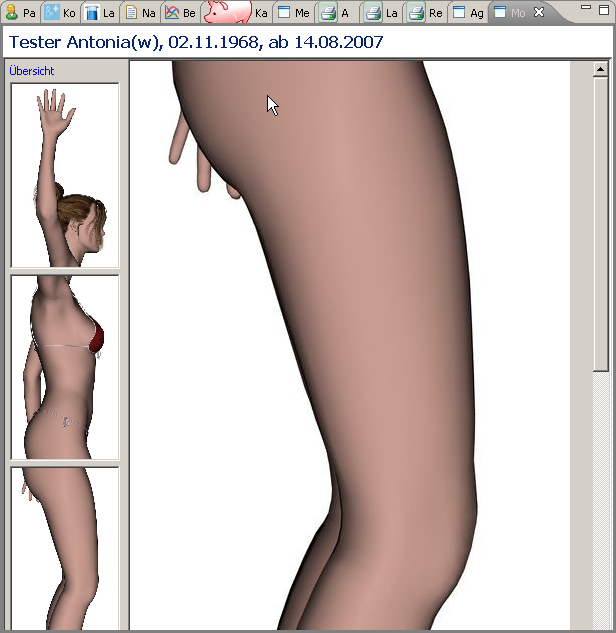
\includegraphics[width=8.5cm]{molemax3}
         \caption{Detailansicht}
         \label{fig:mole3}
     \end{center}
 \end{figure}

Wenn Sie oben auf den Text 'Übersicht' klicken, gelangen Sie wieder zur Übersichtsseite zurück. Wenn Sie auf eines der Detailbilder links klicken, erhalten Sie eine Ansicht dieses Detailbilds in voller Grösse (Das Fenster erhält Scrollbalken, falls das Bild nicht mehr ganz hineinpasst).

\section{Verlaufsbeobachtung erstellen}
Wenn eine verdächtige Läsion über die Zeit beobachtet werden soll, können Sie mit der Maus einen Rahmen um diese Läsion ziehen (einfach mit gedrückter linker Maustaste über die entsprechende Stelle fahren), S. Abb \ref{fig:mole4} und \ref{fig:mole5}.

\begin{figure}[htp]
    \begin{minipage}{0.45\textwidth}
        \centering
        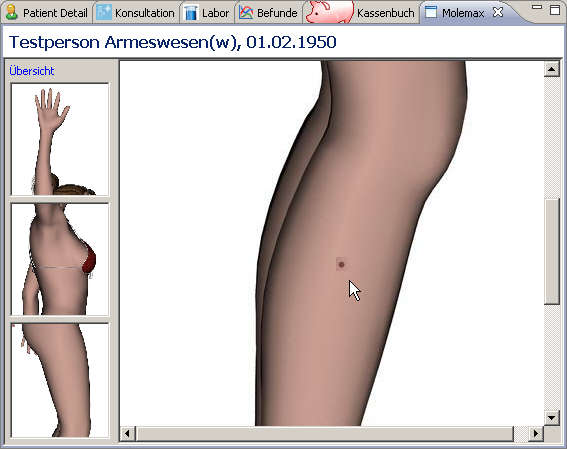
\includegraphics[width=0.9\textwidth]{molemax4}
         \caption{Verdächtige Läsion}
         \label{fig:mole4}
     \end{minipage}
    \hfill
    \begin{minipage}{0.45\textwidth}
        \centering
        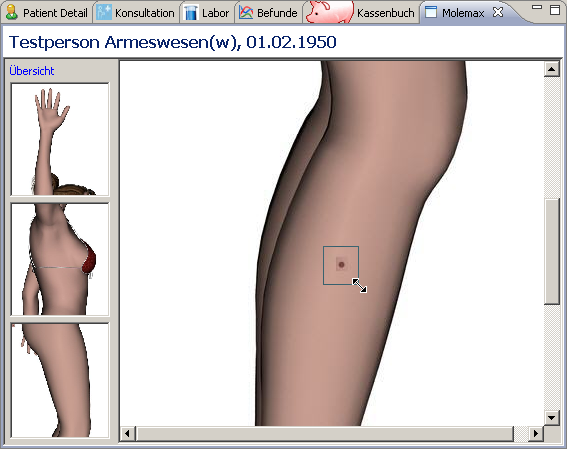
\includegraphics[width=0.9\textwidth]{molemax5}
        \caption{Läsion markieren}
        \label{fig:mole5}
     \end{minipage}
\end{figure}

Es können pro Übersichtsaufnahme beliebig viele, auch überlappende, Regionen auf diese Weise markiert werden. Wichtig: Molemax gibt diesen Regionen keinerlei spezielle Bedeutung, sondern nur die Information Grösse und Position relativ zum Gesamtbild. Ob Sie damit einen Nävus einrahmen, eine Narbe, einen Operationssitus oder ein Stück Luft neben dem Motiv, ist Molemax egal.

\bigskip

Sie können jetzt aber in diese eingerahmten Felder beliebig viele Detailaufnahmen ziehen. Üblicherweise werden das vergrösserte oder höher aufgelöste Bilder der interessierenden Läsion sein, aber auch hier: Molemax wird jedes Bild, das Sie in einen solchen Rahmen ziehen, der betreffenden Region zuordnen. Das System kann also nicht erkennen, ob Sie die Zuordnung korrekt gemacht haben. \footnote{Sie können einen Rahmen mitsamt einem ggf. darin enthaltenen Bild wieder entfernen, indem Sie mit der rechten Maustaste drauf klicken und aus dem Menu 'Löschen' wählen.}

Jede dieser Detailaufnahmen wird mit dem Aufnahmedatum markiert; bei der Übersichtsdarstellung sehen Sie jeweils nur die neueste Aufnahme.

 \begin{figure}[htp]
     \begin{center}
         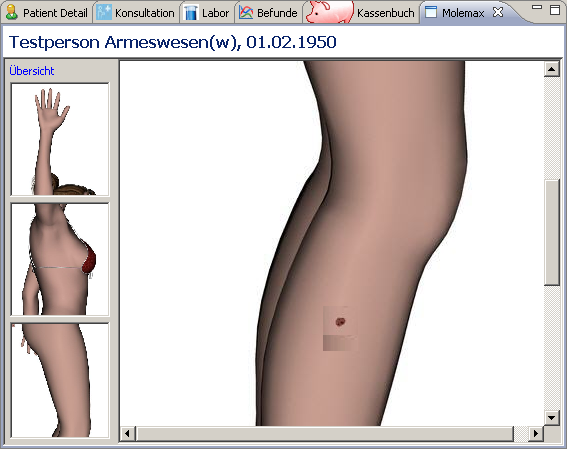
\includegraphics[width=8cm]{molemax6}
         \caption{Einige Detailaufnahmen hineinkopiert}
         \label{fig:mole6}
     \end{center}
 \end{figure}

\clearpage

\section{\glqq Zeitmaschine\grqq}
\begin{wrapfigure}{l}{7cm}
    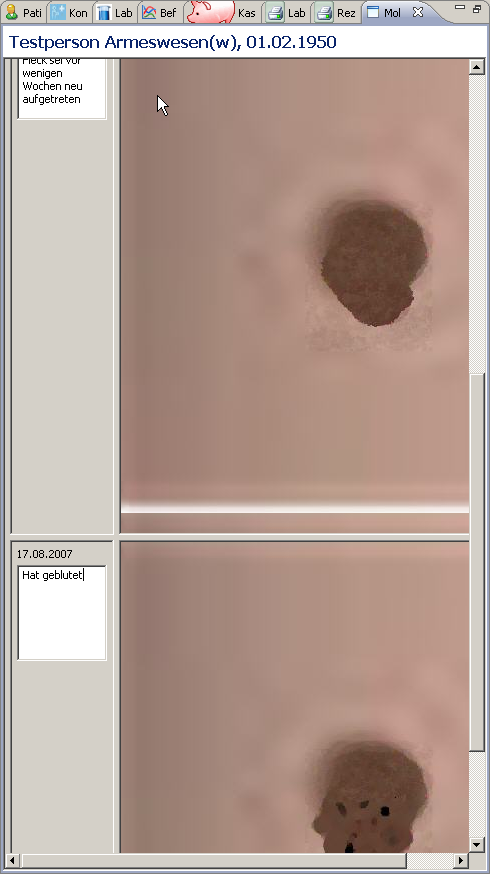
\includegraphics[width=7cm]{molemax7}
    \caption{Zeitmaschine}
\end{wrapfigure}
Wenn Sie auf eine solche Verlaufsbeobachtung doppelklicken, dann erscheinen die Detailaufnahmen in Originalgrösse, alle untereinander, so dass Sie mit dem Scrollbalken in der Zeit vor und zurückfahren können. Sie können zu jeder Aufnahme auch Bemerkungen im Textfenster links eingeben. Die Bemerkungen werden gespeichert, wenn Sie das Textfenster verlassen.
Oben links in der Zeitmaschine finden Sie einen Link \glqq zurück\grqq, mit dem Sie wieder zur Detailansicht zurückkommen.

\section{Mehrere Sequenzen}
Wie eingangs erwähnt, besteht eine einzelne Sequenz aus 12 Aufnahmen, welche natürlich alle zum selben Zeitpunkt aufgenommen sein sollten, sowie Ausschnittsaufnahmen zu beliebigen späteren Zeitpunkten. Manchmal will man aber längere Zeit später erneut eine Basissequenz aufnehmen und von dieser aus eine neue Beobachtungsserie erstellen. Wenn Sie versuchen, ein Bild einer Basissequenz gegen eines zu ersetzen, welches mehr als einen Tag neuer ist, dann wird Molemax Sie fragen, ob eine neue Sequenz erstellt werden soll. In aller Regel sollten Sie hier zustimmen, da es meist nicht sinnvoll (und vom Standpunkt der Dokumentation her auch abzulehnen) ist, vorhandene Sequenzen nachträglich zu verändern.

Sie können mit Klick auf das Kalender-Icon in der Werkzeugleiste jederzeit alle zum aktuellen Patienten vorhandenen Sequenzen auflisten und eine davon zur Anzeige auswählen.

Wenn Sie Bilder aus zwei Sequenzen miteinander vergleichen möchten, starten Sie zwei Elexis-Instanzen und legen sie nebeneinander auf den Bildschirm.

\section{Grenzen}
Da die dargestellten Bilder vollständig im Arbeitsspeicher gehalten werden, ist die maximal mögliche Auflösung der Bilder durch den Arbeitsspeicher vorgegeben. Wenn Sie viel mit grossen Bildern arbeiten, empfiehlt es sich, den PC auf 2GB aufzurüsten und Elexis durch einen grösseren -Xmx Eintrag einen grösseren Arbeitsspeicher zuzuweisen. Es ist aber nicht sinnvoll, Bilder mit einer höheren Auflösung einzulesen, als der Bildschirm anzeigen kann. Im Allgemeinen sollte eine Bildgrösse von 1500x1500 Pixeln für die Darstellung auf einem 20"' Monitor nicht überschritten werden. Auf einem kleineren Monitor entsprechend weniger. Von der Bildqualität her ist eine gute Optik (Makrofähigkeit) und eine gute Ausleuchtung wichtiger, als eine hohe Auflösung. Bilder mit 800x600 Pixel werden meistens genügen. Bei vielen Digitalkameras führt eine zu hohe Auflösung eher zu vermehrtem Bildrauschen und damit im Detailbereich schlechterer Bildqualität.

\end{document}

